%% ----------------------------------------------------------------
\chapter{Chosen Design Approaches}
%% ----------------------------------------------------------------


\section{Camera module}
\label{sec:John_chosen_options}

The camera type chosen was a serial camera as described in \ref{sec:Serial_option}. The particular model chosen was uCam (microCam) or the "Camera Module - Serial JPEG TTL" from the "coolcomponents" website.

The feature set of the uCam is as follows:
	\begin{itemize}
		\item It can output images in both RAW and jpeg formats
		\item It can output RAW images at a range of resolutions:
		\begin{itemize}
			\item 80 x 60
			\item 160 x 120
			\item 320 x 240
			\item 640 x 480
			\item 128 x 128
			\item 128 x 96
		\end{itemize}
		\item It can output jpeg images at a range of resolutions:
		\begin{itemize}
			\item 80 x 64
			\item 160 x 128
			\item 320 x 240
			\item 640 x 480
		\end{itemize}
		\item it can output RAW images with a range of colour settings:
		\begin{itemize}
			\item 2bit Gray Scale
			\item 4bit Gray Scale
			\item 8bit Gray Scale
			\item 8bit Colour
			\item 12bit Colour
			\item 16bit Colour
		\end{itemize}
		\item It will auto-detect baud rates from 14400 to 115200
		\item It has selectable baud rates up to 1228800
		\item Small physical size at 32mm x 32mm
		\item Well documented
	\end{itemize}

The camera was chosen because this feature set meets the specification and also allows for additional functionality, such as setting the resolution, if the full feature set is exploited.

\section{Payload/Ground Station Interaction}

\section{Ground Station Image Viewer}

\section{Progressive JPEG Manipulation}

\section{Physical Implementation}

The final, delivered module is a $90mm\times62mm$ PCB. The PCB manufactured 
for the project was done so for free, using Spirit Circuits' "Go Naked"
service \cite{go-naked}. The PCB itself is a "tracks and holes" only service 
- no soldermask or silkscreen is applied. The schematic of the circuit 
delivered is available in Appendix ???, and of the PCB layout in Appendix 
???. A waterproof lacquer will be applied to the PCB to prevent condensation 
from shorting tracks together, and the module itself presented in a 
waterproof container before flight testing.

\begin{figure}[H]
        \centering
        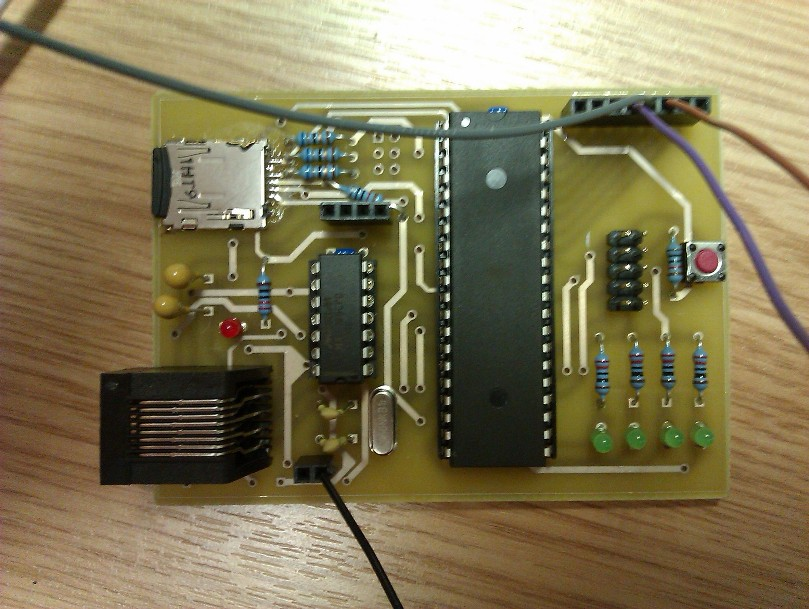
\includegraphics[width=1.00\textwidth]{figures/PayloadImplementation.jpg}
        \captionof{figure}{Image of the final payload, under test, before lacquer is applied. R11 can be seen between the Camera header and a via near the SD card Vcc}
        \label{fig:PayloadImplementation}
\end{figure}

Due to an issue discovered between ordering and receiving the PCB, an 
additional 10k$\Omega$ resistor has been placed between Camera RX and 3V3 (R11 
on the schematic). Also, the Single In Line header holes (for the Port A 
expansion and camera headers) have been widened from 0.40mm to 0.80mm. An 
update to the PCB layout is provided in the delivered repository.

The camera will also be presented in a sealed, weatherproof container.

\section{System Design Overview}

